%% Kanoon-Bridge: full research paper (ACM acmart, sigconf).
%% Compile on Overleaf (acmart is built in): upload this folder; main file kanoon_bridge_acm.tex.
%% Every number is taken from results/tables/ of the repository; docs/PROJECT.md describes each
%% experiment. Items marked \todo{} must be completed before submission.
\documentclass[sigconf,nonacm]{acmart}
%% For submission: \documentclass[sigconf,review,anonymous]{acmart} and fill \acmConference.

\usepackage{booktabs}
\usepackage{multirow}
\usepackage{adjustbox}
\usepackage{tikz}
\usetikzlibrary{positioning,arrows.meta,fit,backgrounds}
\usepackage{xcolor}
\newcommand{\todo}[1]{\textcolor{red}{[TODO: #1]}}
\newcommand{\cmark}{\checkmark}
\newcommand{\ph}{p_{\text{Holm}}}

\settopmatter{printacmref=false}
\setcopyright{none}

\begin{document}

\title{When the Law Is Renumbered: Temporal Misgrounding, Statutory Drift and Verified Retrieval
at India's 2024 Criminal-Code Replacement}

\author{Gaurav Rai}
\affiliation{\institution{\todo{institution}}\city{\todo{city}}\country{India}}
\email{gauravrai2114@gmail.com}

\renewcommand{\shortauthors}{G. Rai}

\begin{abstract}
On 1 July 2024 India replaced its three criminal codes on a single day: the Indian Penal Code
(IPC) by the Bharatiya Nyaya Sanhita (BNS), the Code of Criminal Procedure (CrPC) by the
Bharatiya Nagarik Suraksha Sanhita (BNSS), and the Indian Evidence Act (IEA) by the Bharatiya
Sakshya Adhiniyam (BSA). Sections were renumbered almost everywhere, so a bare section number now
names different provisions in the two codes, and which code governs a case depends on the date
of the incident, not of the search. Legal retrieval and retrieval-augmented generation (RAG)
systems that ignore this \emph{temporally misground} what they return.

We study this replacement end to end. From 1,701 High Court criminal judgments we show that the
transition is slow: through 2025, only 10--29\% of judgments a month cite the BNS while 25--35\%
still cite the IPC. We introduce \emph{statutory drift}, a per-provision measure of how far the law
moved, built from clause alignment with cross-code renumbering, a parser for punishments written
in legal English, and mental-state and threshold reading; against two independent gold sources it
detects changed provisions with F1 0.89, where text similarity reaches 0.62 and the official
crosswalk 0.21. We present Kanoon-Bridge, a three-layer system: a version-aware retrieval core in
which old and new provisions share identifiers; a research agent that routes questions, refines
the code family from evidence and verifies the code in force of its statutes; and an answer layer
that \emph{computes} punishments from statute text and verifies every claim. On the IL-PCSR corpus
the agent raises MAP on date-dependent procedure questions from 0.859 to 0.903 and on Hindi and
Hinglish questions from 0.461 to 0.536 ($\ph<0.05$); on the written facts of 995 real bail orders it
doubles MAP over the core (0.047$\to$0.100, $\ph<0.001$). The answer layer states the correct
punishment for 86\% of 273 BNS questions, where an extractive answer does for 6\%, and flags
82--100\% of injected errors with no false alarm on clean answers. Version-aware search finds
BNS-era judgments from IPC-numbered questions (MAP 0.004$\to$0.151). We also report negative
results: drift-aware down-ranking of old precedent, citation voting, and training-free
table-of-contents navigation in the style of STAIR do not improve retrieval. We release the
system, eight benchmarks, an LLM misgrounding harness, and an annotation kit.
\end{abstract}

\keywords{legal information retrieval, temporal retrieval, statute versioning, retrieval-augmented
generation, claim verification, Indian law, Bharatiya Nyaya Sanhita}

\maketitle

%% ===================================================================================== 1
\section{Introduction}

Legal research is a temporal task: the law that governs a case is the law in force when the facts
occurred. Most legal retrieval benchmarks can ignore this because statutes change slowly, one
amendment at a time. Recent work has begun to measure the failure under the name \emph{temporal
misgrounding}, citing the version of a provision in force today when an earlier one applies
\cite{fiscalqa}, and has documented temporal failure modes of statutory question answering
\cite{oldfriend} and of agentic legal search \cite{timetravel}.

India's 2024 replacement of its criminal codes is the extreme case. Three codes were replaced on
one day. About 500 IPC sections map to BNS sections through a many-to-many crosswalk, nearly every
number changed, and some numbers now name different offences: IPC 302 is murder, BNS 302 is not;
``section 84'' is insanity in the IPC and a different provision in the BNS. An incident in June
2024 and one in August 2024 fall under different codes. And the precedent built on the IPC over
160 years transfers to the BNS only where the provision did not change: sedition (IPC 124A) and
its successor BNS 152 are different offences, while murder (IPC 302, BNS 103) is the same law.
Commercial legal RAG tools still hallucinate \cite{magesh2025}; here even a correct citation can be
correct for the wrong date.

We ask four research questions.
\begin{description}
\item[RQ1] How long do the two codes coexist in practice?
\item[RQ2] Can we measure, per provision, how far the law moved, well enough to decide when old
precedent transfers?
\item[RQ3] Can retrieval be made date-correct across colliding numbers, in English, Hindi and
Hinglish, for section lookups and for written facts?
\item[RQ4] Can generated answers be made verifiable, so that a wrong punishment, a wrong section or
the code not in force is caught or never produced?
\end{description}

\paragraph{Contributions.}
\begin{itemize}
\item \textbf{Evidence of a slow transition} (RQ1): monthly citation shares of the old and new
codes in 1,701 High Court criminal judgments, 2023--2025 (\S\ref{sec:shift}).
\item \textbf{Statutory drift} (RQ2): a per-provision drift vector, a taxonomy and a pairwise
carry-over score, validated against two independent gold sources with a held-out split,
significance tests and ablations, for all three code families (\S\ref{sec:drift},
\S\ref{sec:res-drift}).
\item \textbf{Kanoon-Bridge} (RQ3, RQ4): a version-aware retrieval core, a routed and verified
research agent, and a computed, claim-verified answer layer (\S\ref{sec:system}).
\item \textbf{Eight benchmarks} for the transition: colliding numbers, cross-version precedent
search, date-dependent penal and procedure questions, multilingual needs, punishment QA,
facts$\to$charges from real bail orders, and IPC-numbered questions over BNS-era judgments
(\S\ref{sec:data}), plus an LLM misgrounding harness.
\item \textbf{A detector of overruled precedent} from the judgments' own sentences, the court-made
counterpart of statutory drift (\S\ref{sec:treatment}).
\item \textbf{A thorough evaluation} on the full IL-PCSR corpus with Holm-corrected significance
tests and ablations of every component, and \textbf{negative results} that bound what works
(\S\ref{sec:results}, \S\ref{sec:discussion}).
\end{itemize}

%% ===================================================================================== 2
\section{Background: the 2024 replacement}\label{sec:background}

The BNS, BNSS and BSA came into force on 1 July 2024. Offences committed before that date are
tried under the IPC and proceedings pending before it continue under the CrPC; the new codes
apply to later incidents. Three properties make the change hard for retrieval.

\paragraph{Renumbering with collisions.} The BNS has 358 sections against the IPC's 511; sections
were merged (BNS 318 consolidates IPC 415, 417, 418 and 420), split and reordered. 496 IPC--BNS
pairs appear in the government crosswalk, and most numbers that exist in both codes name different
provisions. A query ``punishment under section 84'' is ambiguous without a date.

\paragraph{Partial change of substance.} Many provisions were copied with cosmetic edits
(``Code''$\to$``Sanhita''), many had only their punishment raised (higher fines, community
service as a new punishment), and some changed what must be proved (BNS 152 adds ``purposely or
knowingly'' and new conduct to what was sedition). Whether IPC-era precedent applies depends on
which of these happened.

\paragraph{A long overlap.} Courts decide old cases under the old codes for years. Search and
answers must therefore serve both codes, chosen by the incident date, and bridge them in both
directions.

%% ===================================================================================== 3
\section{Related Work}\label{sec:related}

\paragraph{Legal case and statute retrieval.} Prior-case retrieval has been studied in the COLIEE
competitions \cite{coliee}, the FIRE AILA tracks for Indian law \cite{aila2019}, and in Chinese
law with LeCaRD \cite{lecard}. For India, IL-TUR \cite{iltur} bundles prior-case retrieval
(IL-PCR) and statute identification (ILSI) with other tasks, and IL-PCSR \cite{ilpcsr} provides a
joint corpus for prior-case and statute retrieval over about 20K judgments with 936 statutes, with
lexical, graph-based and LLM re-ranking baselines. ILDC \cite{ildc} and InLegalBERT
\cite{inlegalbert} support judgment prediction and representation learning for Indian law;
LexGLUE \cite{lexglue} benchmarks legal NLU in English. All of these predate the BNS, and none
models a code replacement.

\paragraph{Temporal and versioned legal retrieval.} Point-in-time retrieval over versioned legal
norms has been modelled with FRBR-style component versioning \cite{frbr} and ontology-driven graph
RAG \cite{satgraph}. Temporal statutory QA benchmarks show that LLMs answer with the current law
when an earlier version applies \cite{oldfriend}; FiscalQA Pro names this temporal misgrounding and
finds RAG over a current-version corpus nearly always wrong on earlier-dated questions
\cite{fiscalqa}; reinforcement learning has been used to make agentic legal search time-consistent
\cite{timetravel}. These works study gradual amendment of one code. We study a one-day replacement
of three codes with colliding numbers, where selecting the version is not enough: the right section
of the new code must also be found, and old precedent must be qualified. Mapping datasets between
the old and new Indian codes exist \cite{ieeemapping}; we know of no retrieval or RAG evaluation of
the transition.

\paragraph{Legal change and text comparison.} Comparing versions of legislation is an old task of
legal informatics (consolidation, redlining); we compare across codes rather than versions, with
clause alignment by word-bigram containment \cite{broder1997} after renumbering cross-references, and
add a structured reading of punishments and mental states that similarity measures cannot see.

\paragraph{Retrieval-augmented generation and verification.} RAG grounds generation in retrieved
text, but legal RAG tools still produce unsupported and wrong statements \cite{magesh2025}.
Attribution is evaluated sentence by sentence in ALCE \cite{alce} and atomic-fact precision in
FActScore \cite{factscore}; RARR revises generated text to agree with retrieved evidence
\cite{rarr}; Self-RAG trains a model to retrieve and critique on demand \cite{selfrag}; corrective
RAG evaluates retrieved documents and corrects the retrieval \cite{crag}. Recent legal benchmarks
check citations claim by claim \cite{lephantomcite,parcel}. Our answer layer differs in computing
what can be computed (the punishment) instead of generating it, and in domain-specific checks:
quantities, section identity across codes, the code in force, modal negation, verbatim quotation.

\paragraph{Agentic and adaptive retrieval.} Interleaving reasoning and retrieval (ReAct
\cite{react}, IRCoT \cite{ircot}) and routing by question complexity (Adaptive-RAG
\cite{adaptiverag}) motivate our agent's routing; we fuse sub-query results with reciprocal rank
fusion \cite{rrf} and CombSUM \cite{combsum}, gate pseudo-relevance feedback \cite{lavrenko2001} by
query-performance prediction \cite{cronentownsend2002}, and add a verification step specific to
statutes.

\paragraph{Citation authority and treatment.} Citation networks give authority scores via
PageRank \cite{pagerank}. Commercial citators (Shepard's, KeyCite) label whether a case is still
good law; nothing comparable exists for Indian judgments. Public-defender retrieval studies argue
that case search without validity information is unreliable \cite{publicdefenders}. We mine
treatment from the judgments' own sentences.

\paragraph{Structure-aware retrieval and generative retrieval.} Generative retrieval maps queries
to document identifiers with a trained model \cite{dsi}; STAIR addresses a corpus through its table
of contents rather than length-based chunks and reports gains over DSI and dense retrieval on book
collections \cite{stair}. We test the training-free counterpart for statutes, whose table of
contents (code, chapter, sub-heading, section) is official.

\paragraph{KV-cache reuse for RAG serving.} PagedAttention manages the KV cache in blocks
\cite{vllm}; RAGCache caches the KV states of retrieved documents across requests \cite{ragcache};
CacheBlend reuses them at any position with partial recomputation \cite{cacheblend}; PACT-KV tiers
KV blocks between GPU and CPU memory by a measured cost signal and reports that recency-based
policies fail on RAG traffic \cite{pactkv}. We measure chunk reuse in legal RAG traffic as a
workload study for these systems.

\paragraph{Multilingual and tolerant legal search in India.} Users in India type Hindi in Devanagari
or in Roman script mixed with English (Hinglish). We combine transliteration, a legal lexicon and
phonetic matching; tolerant retrieval follows the textbook treatment of spelling correction and
k-gram wildcards \cite{iir}, evaluated with simulated known-item queries \cite{azzopardi2007}.

%% ===================================================================================== 4
\section{The transition in the courts}\label{sec:shift}

We sampled criminal judgments of five High Courts (Delhi, Allahabad, Punjab and Haryana, Gujarat,
Kerala) from the eCourts Indian High Court Judgments open dataset (CC-BY-4.0), 2023--2025, 12--30
per court and month, 1,701 in total, and extracted every section citation with our code-aware
tokenizer (``u/s 302 IPC'', ``Section 103 of the BNS'', ``BNSS 482'').

No judgment in the sample cites the BNS before October 2024. Through 2025, between 10\% and 29\% of
judgments per month cite the BNS while 25--35\% still cite the IPC (Figure~\ref{fig:shift}); the BNS
share of all penal section mentions ranges from 5\% to 58\% by month. Most pending cases concern
incidents before 1 July 2024, so both codes will be cited for years (\textbf{RQ1}). A retrieval
system must serve both, choose by date, and connect them.

\begin{figure}[t]
\centering
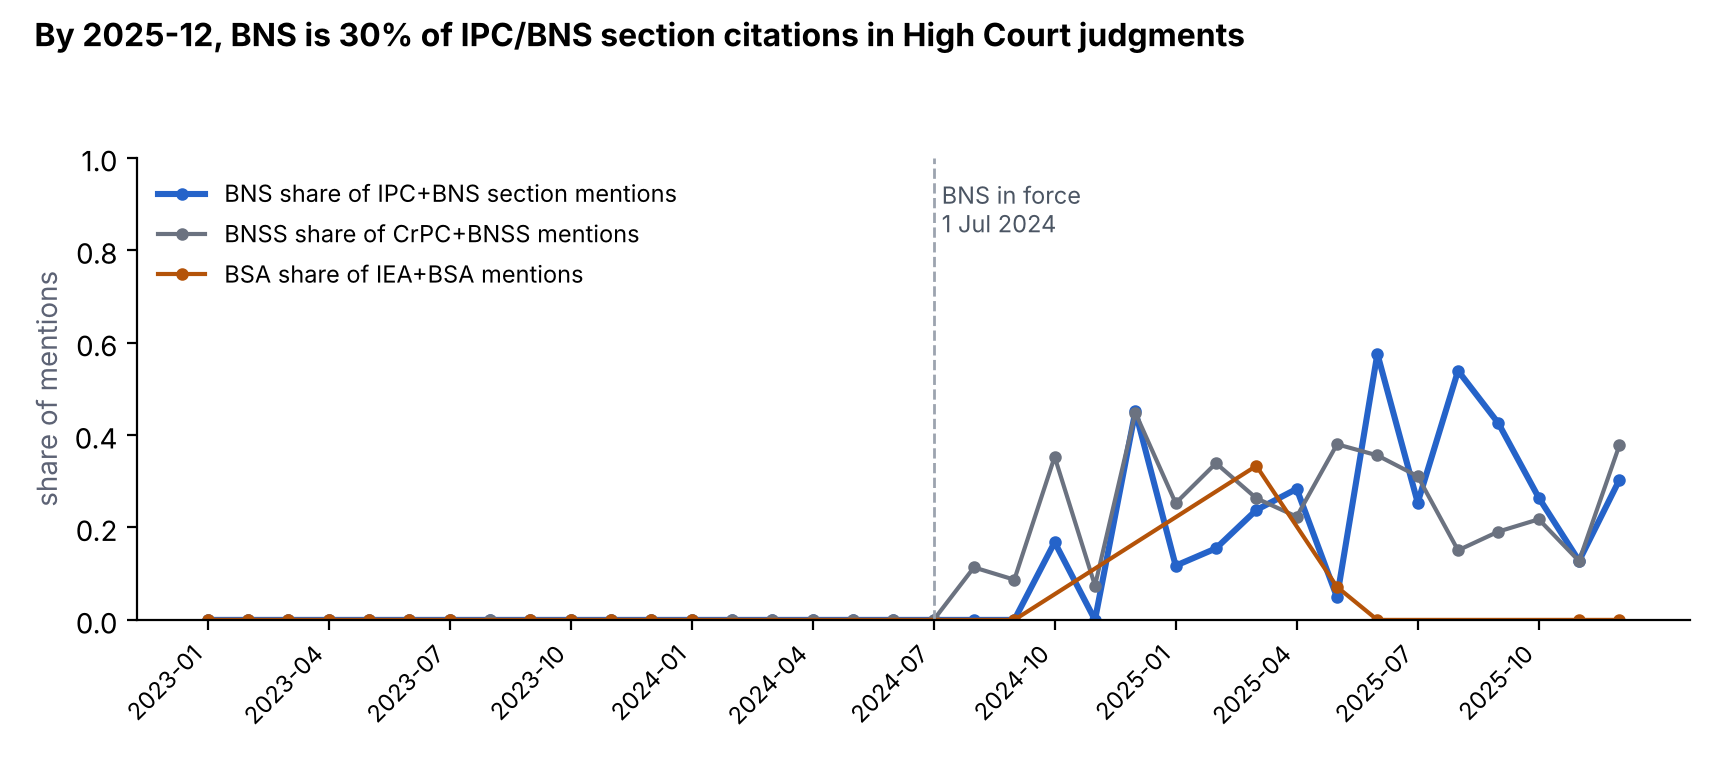
\includegraphics[width=\columnwidth]{figures/citation_shift.png}
\caption{Share of High Court criminal judgments citing the IPC and the BNS, per month (eCourts
open data, 1,701 judgments of five High Courts).}
\label{fig:shift}
\end{figure}

%% ===================================================================================== 5
\section{Data and benchmarks}\label{sec:data}

\paragraph{Corpora.}
\begin{itemize}
\item \textbf{IL-PCSR} \cite{ilpcsr}: 3,183 candidate precedents, 936 candidate statutes (IPC,
CrPC, IEA and others), 5,017 / 627 / 627 train / dev / test query judgments with cited precedents
and statutes. CC-BY-NC-SA; not redistributed.
\item \textbf{New codes}: the 358 BNS sections (bare text from bns-study-platform) and the BNSS and
BSA (India Code). \textbf{Old codes' current text}: India Code's consolidated IPC, CrPC and IEA via
kanoonhq/open-laws (CC0), cleaned of footnotes and State amendments.
\item \textbf{eCourts High Court judgments} (CC-BY-4.0): the 1,701 judgments of \S\ref{sec:shift}.
\item \textbf{IndianBailJudgments-1200} \cite{bail1200} (CC-BY-4.0): 1,200 bail orders with
written facts and charged sections.
\end{itemize}
Our main corpus is IL-PCSR plus the new codes (3,183 precedents, 1,995 statutes); for E10 and a
repetition of E13 we add the eCourts judgments (4,884 precedents). The \emph{open corpus} (all six
codes from India Code, the BNS and the eCourts judgments) needs no restricted data.

\paragraph{Crosswalks.} IPC--BNS: 496 pairs from the government's comparison tables, cross-checked
between the published PDF and a JSON source (468 of 494 agree); offence identifiers group each IPC
section with its BNS successors (343 ids). CrPC--BNSS and IEA--BSA: aligned by text similarity
(698 shared provision ids), flagged as automatic.

\paragraph{Benchmarks.} Table~\ref{tab:benchmarks} lists the evaluation sets. E1 is IL-PCSR's own
test split. E2--E10 are generated from the crosswalks, IL-PCSR citations and the eCourts
judgments; E4 and E6 are written and judged by hand with a second, declared AI judge; E14 uses an
independent punishment summary as gold; E19 uses a third-party dataset.

\begin{table*}[t]
\centering\small
\caption{Evaluation sets. ``Gold'' is the relevance source.}
\label{tab:benchmarks}
\begin{adjustbox}{max width=\linewidth}
\begin{tabular}{llrll}
\toprule
Set & Task & Queries & Gold & Tests \\
\midrule
E1 & judgment $\to$ cited precedents / statutes (E1s) & 627 & IL-PCSR citations & ranking on pasted cases \\
E1q & first 40 words of the facts $\to$ precedents & 627 & IL-PCSR citations & typed-question proxy \\
E2 & bare colliding number (``section 84'') with a date & 252 & expected section by date & collision resolution \\
E3 / E8 & ``cases under section 103 BNS'' (BNSS/BSA for E8) & 49 / 62 & precedents applying the predecessor & cross-version search \\
E4 & information needs in English, Hindi, Hinglish & 50 (150) & pooled, two judges & multilingual search \\
E6 & topical needs with the user's State & 40 & graded binding / persuasive & jurisdiction \\
E7 & penal provision by name, incident before/after 1 July 2024 & 200 & section of the code in force & date-correct statutes \\
E9 & procedure/evidence provision, before/after & 342 & section of the code in force & date-correct statutes \\
E10 & ``cases under section 503 IPC'' & 39 & 348 BNS-era judgments citing the successor & old numbers $\to$ new judgments \\
E11--E12 & which provisions changed; hazard audit & 346 sections & S1 mapping, S2 notes & statutory drift \\
E13 & BNS-era question per cited new-code section & 185 (378) & IL-PCSR citations & drift in ranking \\
E14 & ``What is the punishment for \ldots?'' & 273 & independent summaries & computed answers \\
E15 & six injected error types in answers & up to 249 each & the injection & claim verification \\
E19 & written facts of bail orders $\to$ charged sections & 995 & charge sheets (dataset) & fact-style questions \\
E20 & E7/E9/E2 asked to an LLM & 120+ & code in force & LLM misgrounding (harness) \\
E21 & overruled / doubted / followed & 116 judgments & legal record & judicial treatment \\
E22 & 2,082 RAG questions & -- & -- & KV-cache reuse \\
\bottomrule
\end{tabular}
\end{adjustbox}
\end{table*}

%% ===================================================================================== 6
\section{System architecture}\label{sec:system}

Figure~\ref{fig:arch} shows Kanoon-Bridge. An offline build ingests the corpora, segments judgments
into rhetorical zones, extracts metadata (court, State, date, cited sections), builds the
crosswalks and offence identifiers, the indexes, the citation graph and the drift tables. Online,
three layers answer a question: the retrieval core, the research agent and the answer layer.

\begin{figure*}[t]
\centering
\begin{adjustbox}{max width=\textwidth}
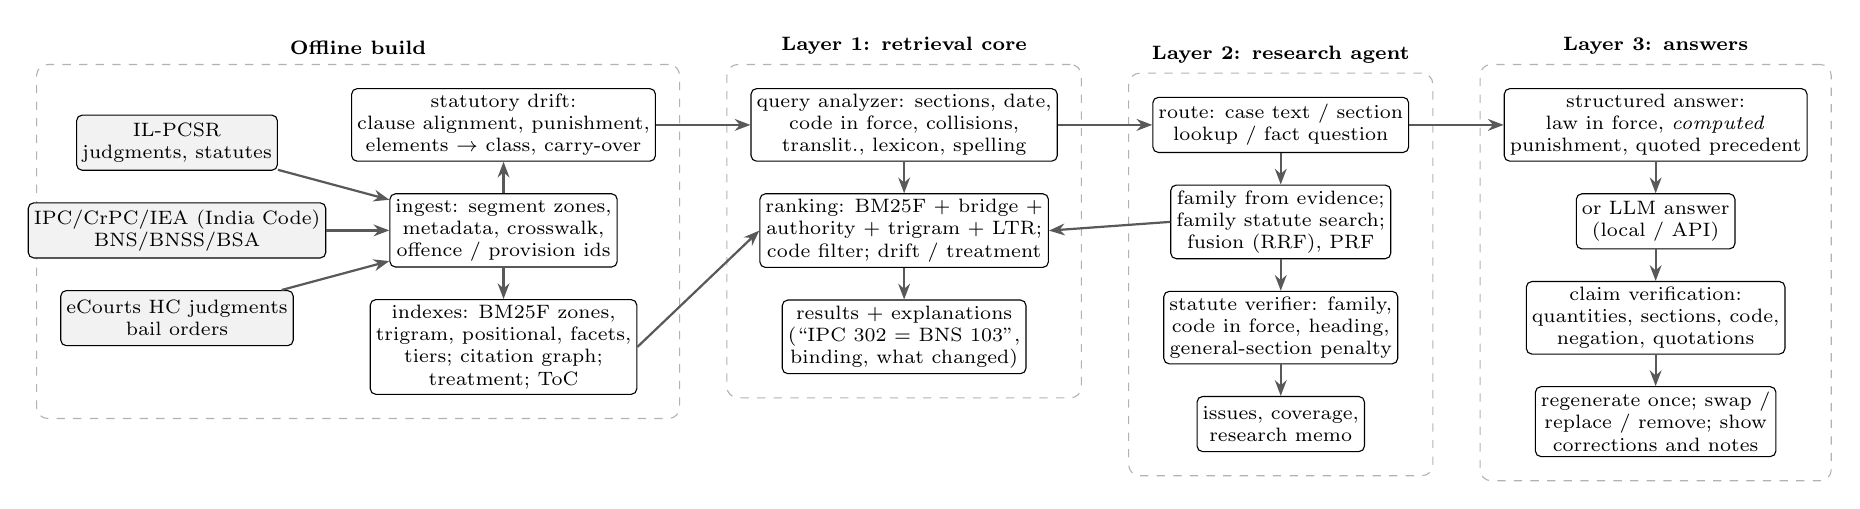
\begin{tikzpicture}[
  node distance=4mm and 6mm,
  box/.style={draw, rounded corners=2pt, align=center, font=\scriptsize, minimum height=7mm, inner sep=2pt, fill=white},
  data/.style={box, fill=gray!10},
  layer/.style={draw=gray!60, dashed, rounded corners=4pt, inner sep=3mm},
  arr/.style={-{Stealth[length=2mm]}, thick, gray!70!black}]
% offline build
\node[data] (ilpcsr) {IL-PCSR\\judgments, statutes};
\node[data, below=of ilpcsr] (codes) {IPC/CrPC/IEA (India Code)\\BNS/BNSS/BSA};
\node[data, below=of codes] (hc) {eCourts HC judgments\\bail orders};
\node[box, right=of codes, xshift=2mm] (ingest) {ingest: segment zones,\\metadata, crosswalk,\\offence / provision ids};
\node[box, above=of ingest] (drift) {statutory drift:\\clause alignment, punishment,\\elements $\to$ class, carry-over};
\node[box, below=of ingest] (index) {indexes: BM25F zones,\\trigram, positional, facets,\\tiers; citation graph;\\treatment; ToC};
% core
\node[box, right=12mm of drift] (analyze) {query analyzer: sections, date,\\code in force, collisions,\\translit., lexicon, spelling};
\node[box, below=of analyze] (rank) {ranking: BM25F + bridge +\\authority + trigram + LTR;\\code filter; drift / treatment};
\node[box, below=of rank] (present) {results + explanations\\(``IPC 302 = BNS 103'',\\binding, what changed)};
% agent
\node[box, right=12mm of analyze] (route) {route: case text / section\\lookup / fact question};
\node[box, below=of route] (family) {family from evidence;\\family statute search;\\fusion (RRF), PRF};
\node[box, below=of family] (verify) {statute verifier: family,\\code in force, heading,\\general-section penalty};
\node[box, below=of verify] (memo) {issues, coverage,\\research memo};
% answer
\node[box, right=12mm of route] (struct) {structured answer:\\law in force, \emph{computed}\\punishment, quoted precedent};
\node[box, below=of struct] (llm) {or LLM answer\\(local / API)};
\node[box, below=of llm] (claims) {claim verification:\\quantities, sections, code,\\negation, quotations};
\node[box, below=of claims] (correct) {regenerate once; swap /\\replace / remove; show\\corrections and notes};
\begin{scope}[on background layer]
\node[layer, fit=(ilpcsr)(hc)(drift)(index), label={[font=\scriptsize\bfseries]above:Offline build}] {};
\node[layer, fit=(analyze)(present), label={[font=\scriptsize\bfseries]above:Layer 1: retrieval core}] {};
\node[layer, fit=(route)(memo), label={[font=\scriptsize\bfseries]above:Layer 2: research agent}] {};
\node[layer, fit=(struct)(correct), label={[font=\scriptsize\bfseries]above:Layer 3: answers}] {};
\end{scope}
\draw[arr] (ilpcsr) -- (ingest); \draw[arr] (codes) -- (ingest); \draw[arr] (hc) -- (ingest);
\draw[arr] (ingest) -- (drift); \draw[arr] (ingest) -- (index);
\draw[arr] (drift) -- (analyze); \draw[arr] (index.east) -- (rank.west);
\draw[arr] (analyze) -- (rank); \draw[arr] (rank) -- (present);
\draw[arr] (analyze) -- (route); \draw[arr] (route) -- (family); \draw[arr] (family) -- (verify); \draw[arr] (verify) -- (memo);
\draw[arr] (family.west) -- (rank.east);
\draw[arr] (route) -- (struct); \draw[arr] (struct) -- (llm); \draw[arr] (llm) -- (claims); \draw[arr] (claims) -- (correct);
\end{tikzpicture}
\end{adjustbox}
\caption{Kanoon-Bridge. The offline build feeds three online layers; every layer can be used alone
(CLI, web app, Python API). Layer 2 issues its sub-queries to layer 1; layer 3 answers from layer
2's (or layer 1's) results.}
\label{fig:arch}
\end{figure*}

\subsection{Layer 1: version-aware retrieval core}

\paragraph{Version normalisation.} Every IPC section and its BNS successors share an offence
identifier, and every CrPC/IEA provision its BNSS/BSA counterpart. The analyzer adds a query's
section mentions as offence-id terms, so ``section 103 BNS'' matches judgments citing IPC 302; the
same ids drive Boolean search, the statute bridge, similar-case search, learning-to-rank features
and the answer checks.
\paragraph{Date and collisions.} An incident date selects the code in force (before 1 July 2024:
IPC/CrPC/IEA). Statutes are filtered to that code. A bare number is resolved from the date and the
words around it, and the colliding reading is excluded.
\paragraph{Ranking.} Judgments are segmented into facts, arguments, ratio and decision zones; BM25F
\cite{bm25f} scores zones with separate weights. A statute bridge adds the scores of the statutes a
judgment cites; a citation-graph authority prior (PageRank over citations, restricted to the courts
whose rulings bind in the user's State) adds jurisdiction awareness; a word-trigram BM25 channel
carries long case-as-query inputs (IL-PCSR's strongest lexical idea); a linear learning-to-rank
model \cite{liu2009ltr} trained on IL-PCSR's dev split re-ranks the top 100.
\paragraph{Typed queries.} Devanagari is transliterated, Hinglish words are normalised and mapped
through a 165-row legal lexicon, unknown words are corrected against the index vocabulary
(Damerau--Levenshtein with k-gram candidates), and wildcards expand through a k-gram index
\cite{iir}. Tiered indexes and champion lists bound latency.
\paragraph{Explanations.} Each result says why it matched: the offence across codes (``IPC 302 =
BNS 103''), binding or persuasive status for the user's State, what changed in the law, and whether
a later judgment overruled it.

\subsection{Statutory drift}\label{sec:drift}

For a new-code section $b$ and each predecessor $s$, both texts are split into clauses
(sub-sections, items, explanations, exceptions, provisos; illustrations excluded). Cross-references
in the old text are rewritten into the new numbering (also across codes: CrPC text citing IPC
sections), systematic wording updates are normalised away, and each new clause is aligned to its
best old clause by word-bigram containment \cite{broder1997}; a clause below 0.3 is \emph{added} or
\emph{lost}. The drift vector contains:
\begin{itemize}
\item \textbf{retention} (share of old text surviving) and \textbf{novelty} (share of new text),
split into rewording of matched clauses and added clauses, plus absolute inserted-word counts for
short qualifiers (``in parts, at any time during the initial forty days'');
\item \textbf{punishment structure} parsed from legal English: death, life, minimum and maximum
terms (number words included), fine and fine caps, community service; the parser strips
descriptions of \emph{other} offences (``an offence punishable with death'') before reading;
\item \textbf{elements}: mental-state markers (intention, knowledge, ``purposely'', ``dishonestly'')
and quantified thresholds (ages, amounts, periods, head counts);
\item \textbf{structure}: merges and splits, title similarity, length ratio.
\end{itemize}
Hand-set rules map the vector to classes (identical, cosmetic, restructured, punishment,
substantive, new, repealed, unverified). A pairwise carry-over score encodes how much of $s$'s
precedent applies to $b$:
\begin{align*}
c_{\text{guilt}} &= \text{ret}\cdot(1-0.5\,\text{rew})\cdot(1-0.15\,\text{add})\\
&\quad\cdot 0.6^{[\text{mens rea}]}\cdot 0.7^{[\text{threshold}]}\\
c_{\text{sent}} &= c_{\text{guilt}}\cdot 0.5^{[\text{punishment}]}\\
c &= 0.85\,c_{\text{guilt}} + 0.15\,c_{\text{sent}}.
\end{align*}
The weights encode legal judgement (rewording of a clause a precedent read matters more than a
clause added beside it; a punishment change affects sentencing reasoning only) and are not fitted to
the gold labels. When a BNS section merges several IPC sections, each clause is credited to the
predecessor it matches best. A logistic-regression variant, trained on the dev half, predicts
``changed'' from the same vector. In ranking, for a BNS-era question an IPC-era precedent citing
$s$ is down-weighted by $\mu(1-c)$ times the score spread when $c<0.85$; in answers, a sentence
citing an old section whose successor changed is flagged.

\subsection{Layer 2: research agent}

The v1 agent (a rule planner of cross-code, Boolean, facet and statutes-first sub-queries, fused
with RRF, with a QPP-gated pseudo-relevance-feedback round) is our agent baseline. The v2 agent:
\begin{enumerate}
\item \textbf{routes} the question: a pasted judgment ($>$50 words: no feedback, case text
down-weighted), a section lookup, or a fact question \cite{adaptiverag};
\item \textbf{chooses the code family} (penal, procedure, evidence) by cue words, then
\emph{refines it from evidence}: the codes of the top retrieved statutes and the codes the
retrieved precedents cite;
\item runs a \textbf{family statute search} restricted to the family's code in force;
\item adds \textbf{citation votes} for statutes cited by several retrieved precedents, gated off
when a top statute's heading already matches the question;
\item \textbf{verifies} the top statutes: family match, code in force, stemmed heading specificity
against the spelling-corrected question (headings read from the statute text when a source's
titles are bare), and a penalty for definition and general-explanation sections;
\item for fact questions, splits the chosen statute into sub-section \textbf{issues}, looks for each
issue's key terms in the retrieved precedents, searches again for uncovered issues, and writes a
\textbf{research memo} (law in force, counterpart, punishment, what changed, issue coverage).
\end{enumerate}
An optional \textbf{table-of-contents navigation} step (inspired by STAIR \cite{stair}) reads the
codes as a table of contents (code$\to$chapter$\to$Gazette sub-heading$\to$section heading, from
India Code), chooses the chapters whose entry best matches the question, and favours their
sections; it is off by default (\S\ref{sec:res-toc}).

\subsection{Layer 3: computed and verified answers}

\paragraph{Structured answer.} The answer names the top retrieved statute of the code in force with
its heading, \emph{computes} its punishment per sub-section with the drift punishment parser
(never merging different sub-sections' terms into one range), and quotes the best-matching sentence
of the top precedent. The counterpart section, what changed and transfer warnings are shown as
notes, apart from the answer. With an LLM (any OpenAI-compatible server, or an API), the LLM
answers from the numbered sources under a date-aware prompt instead.
\paragraph{Claim verification.} Every sentence is checked against the full text of its cited source:
(i) support by idf-weighted cosine, or, for a sentence stating a punishment, structural agreement
with the source's parsed punishment; (ii) every quantity (years, rupees, days) must appear in the
source; (iii) every section named must be the source's own, cited by it, or its crosswalk
counterpart; (iv) the code must be in force on the incident date; (v) a modal negation the source
lacks, or one the claim drops while restating the source sentence, is a contradiction; (vi)
quotations must be verbatim.
\paragraph{Correction.} An LLM answer with failing claims is regenerated once with the problems
listed. Remaining failures are repaired deterministically: old-code sections are swapped to their
counterparts in force (and re-verified), contradicted sentences are replaced by the source's own
words, unsupported sentences are removed; every action is shown.

\subsection{Judicial treatment}\label{sec:treatment}

Precedent can also be made stale by a court. Indian judgments state treatment in their own words,
most regularly in headnotes (``Sita Ram Goel v. The Municipal Board, [1959] SCR 1148,
overruled.''). Over abbreviation-aware sentences of the precedent pool and the \emph{training}
queries only, we find treatment cues (overruled, per incuriam, no longer good law; doubted,
disapproved; followed, relied on, approved), attach each cue to the case it governs (the case right
after ``overruled (the decision) in'', or a case named shortly before with nothing in between that
could be the real object; never across ``in view of'', ``this Court'', ``the provisions of'', or a
negation), and link the case name to a corpus judgment by party names. A judgment is
\emph{overruled} if a strong negative comes from a judgment decided on or after it. Overruled
judgments are down-weighted in ranking and explained.

%% ===================================================================================== 7
\section{Experimental setup}\label{sec:setup}

\paragraph{Metrics.} MAP, MRR, nDCG@10 and P@1; for E1, IL-PCSR's protocol of macro-F1@$k$ with $k$
chosen on the dev split. Statute-level sets (E2, E7, E9) are also scored by reference: the right
section of the right code at rank 1 (\emph{both@1}). E19 is scored code-blind (an IPC section or its
BNS counterpart counts). Answer-level metrics are defined with each experiment.
\paragraph{Significance.} Paired randomization tests (10,000 sign flips) on per-query AP (and RR or
hit@1), with bootstrap 95\% confidence intervals \cite{smucker2007}, Holm-corrected over all
comparisons of an experiment \cite{holm1979}; McNemar's exact test for paired classifiers
\cite{dietterich1998}; Cohen's $\kappa$ for agreement \cite{cohen1960}.
\paragraph{Splits and tuning.} Learning-to-rank weights and thresholds are fitted on IL-PCSR's dev
split; drift thresholds and the drift classifier on a dev half of the sections (split by a hash of
the section number); nothing is tuned on a test set, and the exceptions found during the work are
declared where they appear (\S\ref{sec:limits}).
\paragraph{Generators.} All answer results use the structured (offline) generator; no LLM was
called (E20 is a harness, \S\ref{sec:res-llm}).

%% ===================================================================================== 8
\section{Results}\label{sec:results}

\subsection{Core retrieval on IL-PCSR (E1)}

Table~\ref{tab:e1} compares the core with unigram BM25 and with IL-PCSR's strongest lexical
baseline, BM25 over word trigrams, run by us. On pasted judgments the core reaches MAP 0.414 against
0.220 for BM25; the gain is the trigram channel (Table~\ref{tab:ablation}), and over the trigram
baseline itself the difference is not significant ($+0.005$, $p=0.34$). On statutes and on
40-word typed-question proxies the core is significantly better ($+0.035$ and $+0.013$ MAP). The
IL-PCSR paper's trained models remain ahead on E1 (Para-GNN with BM25: 0.502 MAP; GPT-4.1
re-ranking: 0.544 on precedents \cite{ilpcsr}); our contribution is not E1 but the transition.

\begin{table}[t]
\centering\small
\caption{E1 on IL-PCSR's test split (627 judgments). The 3-gram baseline is IL-PCSR's; the
paper's published values in brackets.}
\label{tab:e1}
\begin{adjustbox}{max width=\linewidth}
\begin{tabular}{llccc}
\toprule
Set & System & MAP & F1@$k$ & MRR \\
\midrule
\multirow{3}{*}{precedents} & BM25 & .220 & .151 & .316 \\
 & BM25 3-gram [paper] & .409 [.434] & .306 [.322] & .548 [.575] \\
 & Kanoon-Bridge & \textbf{.414} & \textbf{.308} & \textbf{.560} \\
\midrule
\multirow{3}{*}{statutes} & BM25 & .149 & .118 & .281 \\
 & BM25 3-gram [paper] & .185 [.194] & .170 [.178] & .384 [.417] \\
 & Kanoon-Bridge & \textbf{.220} & \textbf{.189} & \textbf{.449} \\
\midrule
typed (E1q) & BM25 / 3-gram / ours & \multicolumn{3}{c}{.051 / .046 / \textbf{.059} (.076 short-query LTR)} \\
\bottomrule
\end{tabular}
\end{adjustbox}
\end{table}

\paragraph{Ablation ladder.} Table~\ref{tab:ablation} adds one component at a time. On pasted
judgments the trigram channel carries the gain (0.220$\to$0.409); the statute bridge and authority
cost 0.02 together; the learned re-ranker recovers it (0.414). On typed proxies the short-query
re-ranker matters most (0.059$\to$0.076). On colliding numbers (E2), version normalisation alone
\emph{hurts} (0.902$\to$0.829: it matches both readings of a number), and the code filter repairs it
(0.885): the two belong together.

\begin{table}[t]
\centering\small
\caption{Ablation ladder (MAP); each row adds one component.}
\label{tab:ablation}
\begin{adjustbox}{max width=\linewidth}
\begin{tabular}{lccc}
\toprule
Step & E1 & E1q & E2 \\
\midrule
BM25 & .220 & .051 & .902 \\
+ trigram channel & .409 & .056 & .902 \\
+ version normalisation & .409 & .056 & .829 \\
+ zones & .409 & .055 & .829 \\
+ code filter & .409 & .055 & .885 \\
+ statute bridge & .383 & .053 & .885 \\
+ authority & .387 & .057 & .885 \\
+ jurisdiction & .388 & .059 & .885 \\
+ learning to rank & .414 & .059 & .885 \\
+ short-query LTR & .414 & \textbf{.076} & .885 \\
\bottomrule
\end{tabular}
\end{adjustbox}
\end{table}

\paragraph{Languages, typos and efficiency.} On E4 (50 needs, each in English, Hindi and Hinglish),
the lexicon is the step that matters: MAP 0.184 without the typed-query steps, 0.186 with
transliteration, 0.457 with the lexicon, 0.461 with phonetic matching (Figure~\ref{fig:lang}).
Second-judge agreement on E4 is $\kappa=0.54$; on E6 it is $-0.16$, because E6's citation-derived
gold and a reader's judgement of topical relevance differ. On 300 simulated misspelled known-item
statute queries \cite{azzopardi2007}, spelling correction recovers MRR@10 from 0.830 to 0.905
(clean: 0.947); through agent v2, from 0.751 to 0.844 (clean 0.914). Champion lists keep Recall@20
at 0.990 of exhaustive scoring at the same median latency (109 vs 111 ms); static tiers halve
latency (59 ms) but keep only 0.245 of the exhaustive top 20, so they stay off.

\begin{figure}[t]
\centering
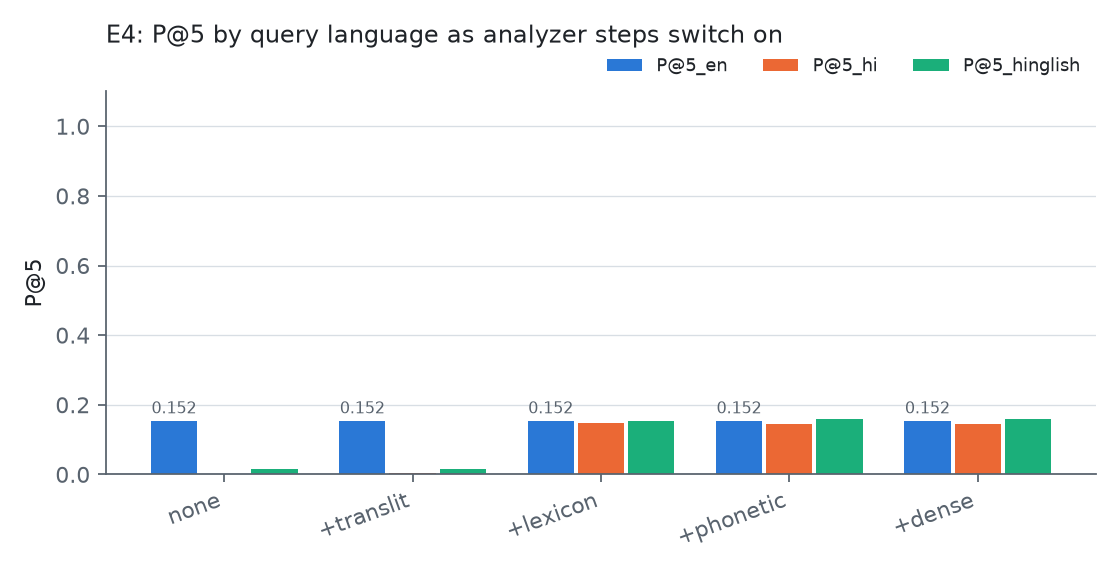
\includegraphics[width=\columnwidth]{figures/language_e4.png}
\caption{E4: MAP as the typed-query steps are added (150 queries: 50 needs in three languages).}
\label{fig:lang}
\end{figure}

\subsection{Version-aware retrieval (E2, E3, E7--E10)}

Table~\ref{tab:version} shows the core against BM25 on the sets that depend on the replacement. A
question in new-code numbers finds precedents decided under the old code (E3: 0.006$\to$0.655 MAP;
E8 for procedure and evidence: 0.005$\to$0.654), and IPC-worded controls also improve (0.503$\to$0.769),
so the gain is not a numbering artefact. Questions by provision name with a date get the right code
at rank 1 in 95\% of cases (BM25: 48\%). On colliding numbers no wrong-offence section reaches the
top 10 (BM25: 7.5\% of queries). On E10, with the eCourts judgments indexed, IPC-numbered questions
find BNS-era judgments (0.004$\to$0.151 MAP; 32 wins, 2 losses, $p<0.001$): plain BM25 cannot
connect ``section 503 IPC'' to a judgment citing BNS 351 (\textbf{RQ3}).

\begin{table}[t]
\centering\small
\caption{Version-dependent sets: BM25 vs the core. All differences except E2's MAP are significant
($\ph<0.05$).}
\label{tab:version}
\begin{adjustbox}{max width=\linewidth}
\begin{tabular}{llcc}
\toprule
Set & Metric & BM25 & Core \\
\midrule
E3 asked in BNS numbers & MAP & .006 & \textbf{.655} \\
E3 control, IPC numbers & MAP & .503 & \textbf{.769} \\
E8 asked in BNSS/BSA numbers & MAP & .005 & \textbf{.654} \\
E7 penal, by date & MAP & .645 & \textbf{.880} \\
E7 right code at rank 1 & acc. & .475 & \textbf{.955} \\
E9 procedure, by date & MAP & .630 & \textbf{.859} \\
E2 colliding numbers & wrong hit@10 & 7.5\% & \textbf{0\%} \\
E6 jurisdiction & nDCG@10 & .366 & \textbf{.657} \\
E10 IPC numbers $\to$ BNS-era & MAP & .004 & \textbf{.151} \\
\bottomrule
\end{tabular}
\end{adjustbox}
\end{table}

\subsection{Statutory drift (E11--E12)}\label{sec:res-drift}

\paragraph{Gold.} S1 is a section-level retained/changed mapping; S2 is the change notes of an
independent study platform, read into categories (unchanged, structure, punishment, substance) by
our rules. On the 346 BNS sections with an IPC predecessor they agree at $\kappa=0.75$: ``did it
change?'' has more than one defensible answer.

\paragraph{E11a: which provisions changed.} On the held-out half (Table~\ref{tab:drift}), the
hand-set drift rules reach F1 0.85 on S1 and the learned model 0.89 ($\kappa$ 0.85), against 0.62
for the best text-similarity baseline and 0.21 for the official crosswalk's own relation (McNemar
$p<0.001$ against the crosswalk; bootstrap CIs of the rules and edit similarity do not overlap on
S1: 0.77--0.91 vs 0.53--0.71). On S2, the more independent source, the learned model reaches 0.81
($\kappa$ 0.73). The learned model's agreement with S1 exceeds the two sources' agreement with each
other; we read this as S1 itself being partly text-derived, not as better-than-human performance
(\textbf{RQ2}).

\begin{table}[t]
\centering\small
\caption{E11a: which IPC provisions changed in the BNS (held-out half, 183 sections).}
\label{tab:drift}
\begin{adjustbox}{max width=\linewidth}
\begin{tabular}{lcccc}
\toprule
System & F1 (S1) & $\kappa$ (S1) & F1 (S2) & $\kappa$ (S2) \\
\midrule
crosswalk relation $\neq$ same & .21 & $-$.03 & .32 & .10 \\
edit similarity (dev-tuned) & .62 & .39 & .68 & .45 \\
tf-idf cosine (dev-tuned) & .60 & .34 & .64 & .38 \\
drift rules, hand-set & .85 & .78 & .76 & .65 \\
drift rules, dev-tuned & .84 & .77 & .77 & .66 \\
drift vector + LR & \textbf{.89} & \textbf{.85} & \textbf{.81} & \textbf{.73} \\
\bottomrule
\end{tabular}
\end{adjustbox}
\end{table}

\paragraph{E11b: ablation.} Removing the punishment parser drops F1 on S1 from 0.84 to 0.20: most
BNS changes are raised fines and terms, one-word edits invisible to similarity. Renumbering and
clause alignment add about 0.01 AUC to the carry-over score and make the explanations possible
(``a sub-section was added'', ``section 334 became 122'') without changing detection; the
mental-state reading slightly \emph{hurts} detection (0.853 without it vs 0.843) but catches
``purposely or knowingly'' in BNS 152 and stays for the explanation (Figure~\ref{fig:driftabl}).

\begin{figure}[t]
\centering
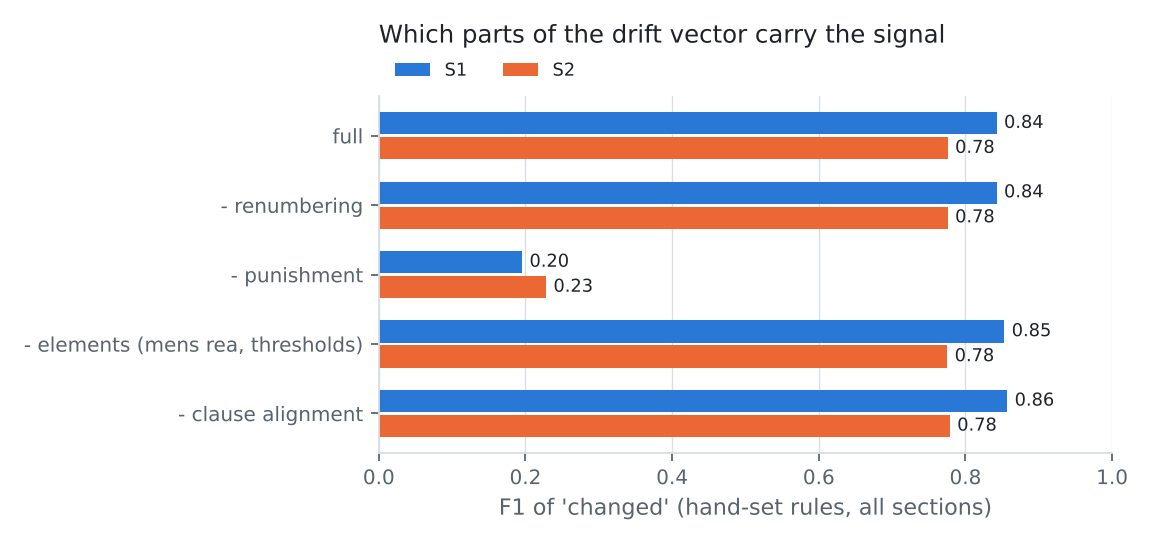
\includegraphics[width=\columnwidth]{figures/drift_ablation.png}
\caption{E11b: change-detection F1 of the hand-set drift rules without each component (all 346
sections).}
\label{fig:driftabl}
\end{figure}

\paragraph{E11c--f.} Against S2's punishment category the punishment comparison reaches precision
0.80, recall 0.90 (F1 0.85, $\kappa$ 0.80). Field by field, the parser on the bare act agrees with
the source's own one-line punishment summaries on 95--100\% of 273 sections (death 95\%, life 97\%,
maximum term 98\%, fine 99.6\%). Repeal detection reaches AUC 0.96 (F1 0.54 vs 0.38 for ``not in the
crosswalk''). Mean carry-over falls from 0.95 for unchanged sections to 0.84--0.89 for changed ones;
it separates change from no change but not substance from punishment.

\paragraph{Procedure and evidence.} For CrPC$\to$BNSS and IEA$\to$BSA (S1 only), edit similarity is
as good as the drift systems (F1 0.78 vs 0.75; 0.53 vs 0.40): without punishments, what is left is
wording. Repeal detection is strong (AUC 0.98 and 0.97). The drift layer remains useful there for
its per-pair carry-over and explanations (for instance, BNSS 187 lets the 15 days of police custody
be taken ``in parts, at any time during the initial forty days or sixty days'').

\paragraph{E12: hazard audit.} 14 of 343 IPC--BNS offence ids equate sections with carry-over below
0.5, among them sedition (124A$\to$152, 0.24) and house-breaking by night (446$\to$330, 0.14);
others are consolidations (general explanations into BNS 3). This is an upper bound for legal
review, not an error count.

\subsection{Drift in ranking (E13)}\label{sec:res-e13}

For one BNS-era question per cited BNS section, we compare the full system with the drift penalty
off and on. On identical and cosmetic sections nothing moves (no harm). On changed sections the
penalty costs citation-MAP (IPC substantive: 0.645$\to$0.508 on IL-PCSR; 0.321$\to$0.224 with the
eCourts judgments) while \emph{stale@10}, the share of the top 10 with transfer below 0.5, was
already near zero (at most 2\% before, 1.5\% with the eCourts judgments). Citation relevance counts a
stale precedent as relevant, and stale precedents are rare at the top: the drift signal is better
\emph{shown} (as a note on the result) than \emph{ranked}. We keep the penalty in the interactive
system as a safety signal and report it as a negative result for ranking.

\subsection{The research agent (E16--E17, E19)}

\paragraph{IL-PCSR corpus (E17, Table~\ref{tab:agent}).} The agent improves the questions about the
law: procedure and evidence by date ($+0.044$ MAP, $\ph=0.04$), Hindi/Hinglish ($+0.075$,
$\ph=0.04$), penal by date ($+0.035$; 28 wins, 8 losses, $\ph=0.18$). On pasted judgments (E1) it
routes to case-text mode and keeps the core's ranking (1.1 searches per query, $-0.002$ MAP), where
the v1 rule-planner agent lost 0.11 MAP ($\ph=0.003$ for v2 over v1). On E6 both agents trade MAP
for the top of the list (P@1 0.80$\to$0.90; all top-5 results binding): their fused sub-queries put
binding judgments first.

\begin{table}[t]
\centering\small
\caption{E17: agent v2 on the IL-PCSR corpus (MAP). $^\dagger$: $\ph<0.05$ vs core (paired
randomization, Holm over 32 comparisons).}
\label{tab:agent}
\begin{adjustbox}{max width=\linewidth}
\begin{tabular}{lccc}
\toprule
Set & Core & Agent v1 & Agent v2 \\
\midrule
E1 judgments $\to$ precedents & \textbf{.414} & .306 & .412$^\dagger$ \\
E1q typed proxies & \textbf{.059} & .056 & .057 \\
E1s judgments $\to$ statutes & \textbf{.220} & .218 & .212 \\
E2 colliding numbers & .885 & \textbf{.936} & .921 \\
E4 Hindi / Hinglish / English & .461 & .460 & \textbf{.536}$^\dagger$ \\
E6 jurisdiction & \textbf{.630} & .554 & .554$^\dagger$ \\
E7 penal, by date & .880 & .877 & \textbf{.915} \\
E9 procedure, by date & .859 & .859 & \textbf{.903}$^\dagger$ \\
\bottomrule
\end{tabular}
\end{adjustbox}
\end{table}

\paragraph{Agent ablations (Table~\ref{tab:agentabl}).} The verifier carries the gains: without it
E7 falls to 0.873 and E9 to 0.845 on IL-PCSR, and both@1 to the core's level on the open corpus.
The family search is mixed on both corpora (it helps E2 and E4, costs E7 and E9). Issue rounds do
not change statute rankings. Citation votes did nothing with eight synthetic precedents and are
harmful with real ones (\S\ref{sec:discussion}).

\begin{table}[t]
\centering\small
\caption{Agent v2 ablations. IL-PCSR: MAP; open corpus with eCourts judgments: E2 expected@1,
E7/E9 both@1.}
\label{tab:agentabl}
\begin{adjustbox}{max width=\linewidth}
\begin{tabular}{lcccccc}
\toprule
 & \multicolumn{3}{c}{IL-PCSR} & \multicolumn{3}{c}{open corpus} \\
\cmidrule(lr){2-4}\cmidrule(lr){5-7}
Variant & E2 & E7 & E9 & E2 & E7 & E9 \\
\midrule
core & .885 & .880 & .859 & .81 & .79 & .75 \\
agent v2 & .921 & .915 & .903 & .79 & .87 & .82 \\
\; $-$ verification & .927 & .873 & .845 & .79 & .79 & .70 \\
\; $-$ family search & .886 & .932 & .938 & .72 & .90 & .87 \\
\; $-$ citation votes & -- & -- & -- & \textbf{.93} & .87 & .82 \\
\; votes not gated & -- & -- & -- & .73 & .75 & .78 \\
\bottomrule
\end{tabular}
\end{adjustbox}
\end{table}

\paragraph{Written facts (E19).} On the first 60 words of the facts of 995 bail orders, with their
charged sections as gold, the agent doubles the core's MAP (Table~\ref{tab:facts}; $+0.053$, 95\% CI
$[0.043, 0.063]$, 195 wins and 49 losses, $\ph<0.001$) and nearly triples hit@1 ($\ph<0.001$). The
absolute numbers are low: bail facts talk about arrest, custody and bail, so the core drifts to
procedure and evidence sections, and the agent's family refinement pulls it back to penal law. E19
was run after every fix of \S\ref{sec:limits} and was not used to make them.

\begin{table}[t]
\centering\small
\caption{E19: written facts of 995 bail orders $\to$ charged sections (code-blind).}
\label{tab:facts}
\begin{adjustbox}{max width=\linewidth}
\begin{tabular}{lcccc}
\toprule
System & R@5 & R@10 & MAP & hit@1 \\
\midrule
Core & .067 & .092 & .047 & .062 \\
Agent v1 & .081 & .109 & .057 & .071 \\
Agent v2 & \textbf{.120} & \textbf{.138} & \textbf{.100} & \textbf{.170} \\
Agent v2 + ToC navigation & .118 & .138 & .099 & .170 \\
\bottomrule
\end{tabular}
\end{adjustbox}
\end{table}

\subsection{Computed and verified answers (E14, E15, E18)}

\paragraph{Punishment QA (E14 / E18b).} For 273 questions ``What is the punishment for
$\langle$BNS heading$\rangle$?'' with a 2025 incident date, the gold is an independent one-line
summary, parsed, and an answer is right only if every field matches (death, life, minimum and
maximum term, fine and caps, community service). An extractive answer quotes the statute's best
sentence, rarely its punishment clause; the computed answer is right for 85--86\% of questions
(93--94\% when the statute is right) on both corpora (Table~\ref{tab:answers}). Most remaining
errors are gold summaries that describe one sub-section only (\textbf{RQ4}).

\begin{table}[t]
\centering\small
\caption{E14 / E18b: punishment QA (273 BNS questions).}
\label{tab:answers}
\begin{adjustbox}{max width=\linewidth}
\begin{tabular}{lccc}
\toprule
System & statute@1 & right punishment & given statute \\
\midrule
\multicolumn{4}{l}{\emph{IL-PCSR corpus}} \\
core + extractive & .912 & .062 & .064 \\
core + computed, verified & .912 & .854 & .936 \\
agent v2 + computed, verified & \textbf{.927} & \textbf{.861} & .929 \\
\multicolumn{4}{l}{\emph{open corpus}} \\
core + extractive & .897 & .051 & .053 \\
core + computed, verified & .897 & .846 & .939 \\
agent v2 + computed, verified & \textbf{.919} & \textbf{.857} & .928 \\
\bottomrule
\end{tabular}
\end{adjustbox}
\end{table}

\paragraph{Error injection (E15 / E18b).} Into each answer with the right statute we inject one
error per type in the sentence that cites the statute, and count the answers on which a checker
raises a new flag. Claim verification catches 82--100\% of each type, against 17--100\% for v1's
cosine-support and code checks, with no false alarm on clean answers on IL-PCSR (1\% on the open
corpus) against 80--84\% for cosine support (Table~\ref{tab:inject}, Figure~\ref{fig:inject}). The
errors are the types the verifier was designed for, so these are upper bounds for real LLM errors.

\begin{table}[t]
\centering\small
\caption{E15/E18b: share of injected errors flagged (IL-PCSR corpus; base: computed answers).}
\label{tab:inject}
\begin{adjustbox}{max width=\linewidth}
\begin{tabular}{lrcc}
\toprule
Injected error & $n$ & cosine + code (v1) & claim verification \\
\midrule
term of years changed & 191 & .30 & \textbf{.89} \\
fine $\times$10 & 65 & .46 & \textbf{1.00} \\
negation flipped & 248 & .30 & \textbf{.83} \\
old-code section, 2025 incident & 242 & 1.00 & 1.00 \\
section number changed & 249 & .34 & \textbf{1.00} \\
another statute's punishment & 249 & .36 & \textbf{.89} \\
\midrule
\emph{false alarm, clean answers} & 249 & .84 & \textbf{.00} \\
\bottomrule
\end{tabular}
\end{adjustbox}
\end{table}

\begin{figure}[t]
\centering
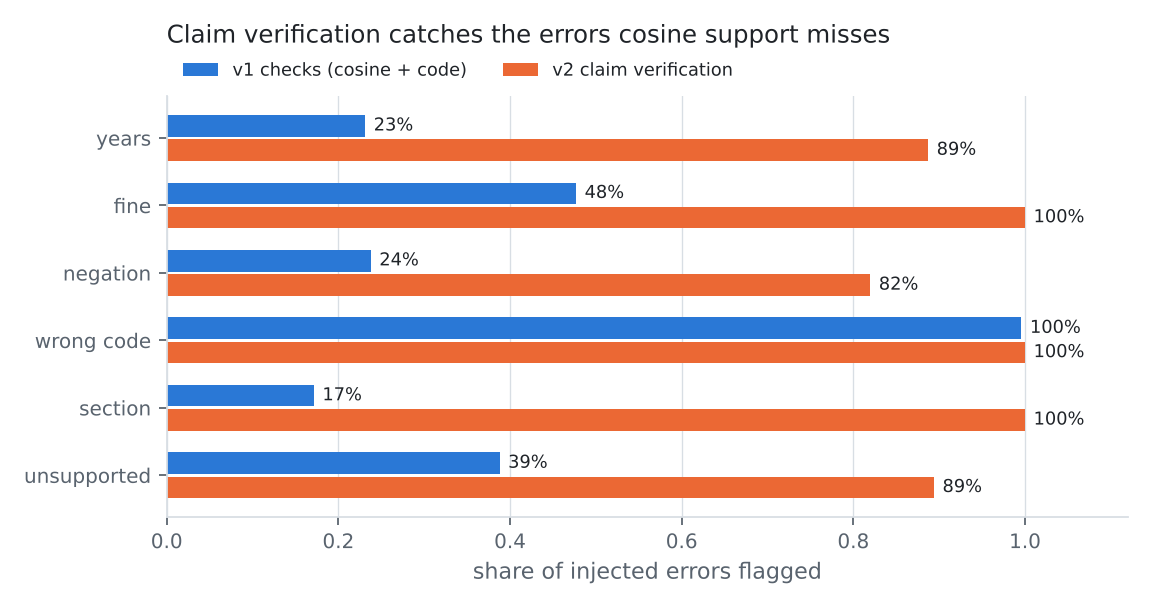
\includegraphics[width=\columnwidth]{figures/layers_error_injection.png}
\caption{Error injection on the open corpus: cosine support vs claim verification.}
\label{fig:inject}
\end{figure}

\paragraph{Hand-written questions (E18a).} On 20 hand-written questions (four unanswerable), the
verified answers carry no old-code section for the incident date (extractive: 0.05 per answer);
both systems abstain on only one of the four unanswerable questions, and the agent also on one
answerable one. Abstention needs work.

\subsection{Judicial treatment (E21)}

From the precedent pool and training queries, 116 judgments receive a treatment and 133 positive
mentions are found; five judgments are flagged overruled: I.~C. Golak Nath v. State of Punjab, State
of Bombay v. United Motors, Northern India Caterers v. State of Punjab, Air India Statutory
Corporation v. United Labour Union, and State of Bombay v. F.~N. Balsara (in part). All five were
overruled; this check is ours against the legal record and is being confirmed by a law student
\todo{annotation result}. An earlier version without the attachment rules flagged ten, half wrongly
(``Devadasan is no longer good law in view of N.~M. Thomas'' was attached to Thomas). Recall is low.
In E1 flagged judgments reach the top 10 for 0.6\% of test queries; demoting them leaves MAP
unchanged: a safety signal for the user, not a ranking gain.

\subsection{Table-of-contents navigation}\label{sec:res-toc}

Choosing chapters by their table-of-contents entries, as STAIR does with a trained generative
retriever \cite{stair}, did not help without training: flat on E7 (both@1 0.890$\to$0.895) and on E19
(MAP 0.0996$\to$0.0989, $\ph=0.82$), worse on E2 (expected@1 0.857$\to$0.762) and E9 (both@1
0.877$\to$0.854). Chapter names are too coarse to choose between neighbouring sections and mislead on
section-number questions; navigation is therefore limited to questions that name no section and
off by default.

\subsection{KV-cache reuse in legal RAG (E22)}

We traced the chunks the answer layer places in the prompt for 2,082 questions (E2, E7, E9, E14,
E19 and the hand-written set, shuffled): 10,036 chunk retrievals of 3,755 distinct chunks. 63\% of
prompt tokens repeat an earlier question's chunk (78\% of statute-chunk tokens, 49\% of precedent
tokens), and the 10\% most frequent chunks take 37\% of retrievals. The working set is large, though:
about 0.65M distinct tokens, or 80\,GiB of Mistral-7B KV (128\,KiB per token). Table~\ref{tab:kv}
simulates chunk-level KV caches (position-independent reuse, as in CacheBlend \cite{cacheblend}).
Frequency beats recency by about 2$\times$, the pattern PACT-KV reports for RAG workloads
\cite{pactkv}; the reuse argues for tiering (hot statute chunks in GPU memory, the long tail in CPU
memory) rather than a larger single cache.

\begin{table}[t]
\centering\small
\caption{E22: share of prompt tokens served from a chunk-KV cache of a given size.}
\label{tab:kv}
\begin{adjustbox}{max width=\linewidth}
\begin{tabular}{rrccc}
\toprule
KV memory & tokens & LRU & LFU & statute-pinned \\
\midrule
0.5 GiB & 4,096 & 1.1\% & 4.4\% & 2.4\% \\
1 GiB & 8,192 & 2.5\% & 7.9\% & 4.7\% \\
2 GiB & 16,384 & 4.8\% & 12.6\% & 8.6\% \\
4 GiB & 32,768 & 9.7\% & \textbf{19.4\%} & 14.6\% \\
$\infty$ & -- & \multicolumn{3}{c}{63\%} \\
\bottomrule
\end{tabular}
\end{adjustbox}
\end{table}

\subsection{LLM temporal misgrounding (E20)}\label{sec:res-llm}

The harness asks one LLM the E7, E9 and E2 questions (balanced across the two sides of 1 July 2024)
under five conditions: closed-book; naive RAG (core retrieval, generic prompt); RAG v1 (date-aware
prompt); RAG v2 (agent, verification, regeneration, correction); and the structured answer without
an LLM. It scores the first section each answer names: the right provision of the code in force,
\emph{misgrounded} (the code not in force, or a colliding number), or no section.
\todo{Run scripts/19\_eval\_misgrounding.py with an open 7--8B model served by vLLM and one API
model; report right@1, misgrounded@1 and any-wrong-code per set and condition in a table here.}

%% ===================================================================================== 9
\section{Discussion}\label{sec:discussion}

\paragraph{What carries the gains.} Three components account for most results: shared
identifiers with a date-based code filter (E2--E10), statute verification in the agent (E7, E9, E17,
E19), and computing rather than generating punishments (E14, E18). None needs training data beyond
IL-PCSR's dev split.

\paragraph{Negative results.} (1) Down-ranking old precedent by carry-over costs citation-MAP
without reducing stale results, which are rare at the top (E13): citation relevance does not reward
legal applicability, so the signal belongs in the explanation. (2) Citation voting promotes the most
cited sections once precedents are real (the open corpus with 1,701 eCourts judgments: $-0.15$ on
E2); we recommend disabling it. (3) Training-free table-of-contents navigation does not help;
STAIR's gains plausibly come from its trained retriever. (4) Outside penal law, plain edit
similarity detects change as well as the drift vector.

\paragraph{Errors found by evaluating on real data.} Two bugs surfaced only on the full corpora and
would have been invisible on synthetic data: IL-PCSR titles its IPC sections ``Section 463 of The
Indian Penal Code, 1860'' with no heading, so the verifier's heading match scored zero and citation
votes promoted the most cited sections (E7 0.810 before the fix, 0.915 after); and on IL-PCSR's
larger vocabulary, wording overlap between a one-line computed punishment and a long statute fell
below the support threshold, so the corrector deleted correct sentences (right punishment 0.31
before the structural check, 0.86 after). Case titles with abbreviations (``Mohd.'', ``THRU. SECY.'')
were split into uncited fragments. We report the fixed numbers and declare the fixes.

\paragraph{Error analysis.} On E14 most remaining failures are gold summaries that describe
one sub-section of a multi-part section. On E19 the facts are written about the bail application,
so procedural vocabulary pulls retrieval towards the BNSS and BSA; the agent's family refinement is
what pulls it back. \todo{a systematic error analysis of E19 and E2 misses by category.}

%% ===================================================================================== 10
\section{Limitations}\label{sec:limits}

\begin{itemize}
\item \textbf{No LLM has been evaluated yet} (E20): the central LLM result is missing.
\item \textbf{Fixes after seeing results.} The statute-heading fix and the structural punishment
support were found by looking at E17/E18; the table-of-contents gate at E2; the citation-vote gate
after the open-corpus E16. E19 and E10 were run after all of them.
\item \textbf{Gold labels.} The drift gold is section-level; S2 is our rule-based reading of
free-text notes; carry-over is validated only indirectly. The treatment check is ours, not a
lawyer's. Human labels are being collected with the released kit.
\item \textbf{Question style.} E7, E9 and E14 are phrased like section headings, which favours
heading matching; E4 and E19 are not.
\item \textbf{Crosswalks.} The procedure and evidence crosswalks are aligned automatically and contain
wrong merges.
\item \textbf{Coverage.} The eCourts sample covers five High Courts; the Supreme Court and other
High Courts may transition at a different pace.
\end{itemize}

\section*{Ethics, licences and reproducibility}
Kanoon-Bridge is a research tool, not legal advice; answers show their sources, corrections and
notes. All data are public court judgments and legislation used under their licences (IL-PCSR
CC-BY-NC-SA; eCourts and IndianBailJudgments-1200 CC-BY-4.0; India Code via open-laws CC0); raw
data are not redistributed. Code, generated benchmarks, result tables and the annotation kit are
released \todo{repository URL}; every number in this paper is produced by a script listed in the
repository. AI assistance was used in implementing and documenting the system and is declared in
the repository's AI-use log; the second judge for E4/E6 is an AI and is reported as such.

\section{Conclusion}
A code replacement turns legal retrieval into a temporal problem with colliding identifiers and a
partial transfer of precedent. Shared identifiers with date-based code selection, verification of
the statutes an agent returns, and computed, claim-checked answers make a measurable difference on
real data; down-ranking old precedent, voting by citations and training-free navigation do not.
Courts will cite both codes for years; the system and benchmarks we release make the transition
measurable, and the LLM harness is ready to measure how often today's models misground.

\begin{acks}
\todo{Acknowledge the annotator(s) and teammates on the course project (Kashvi Tak, Sharanya Gupta,
Shaurya) as appropriate.}
\end{acks}

\bibliographystyle{ACM-Reference-Format}
\bibliography{references}

\end{document}
